
\begin{figure}[ht]
\centering
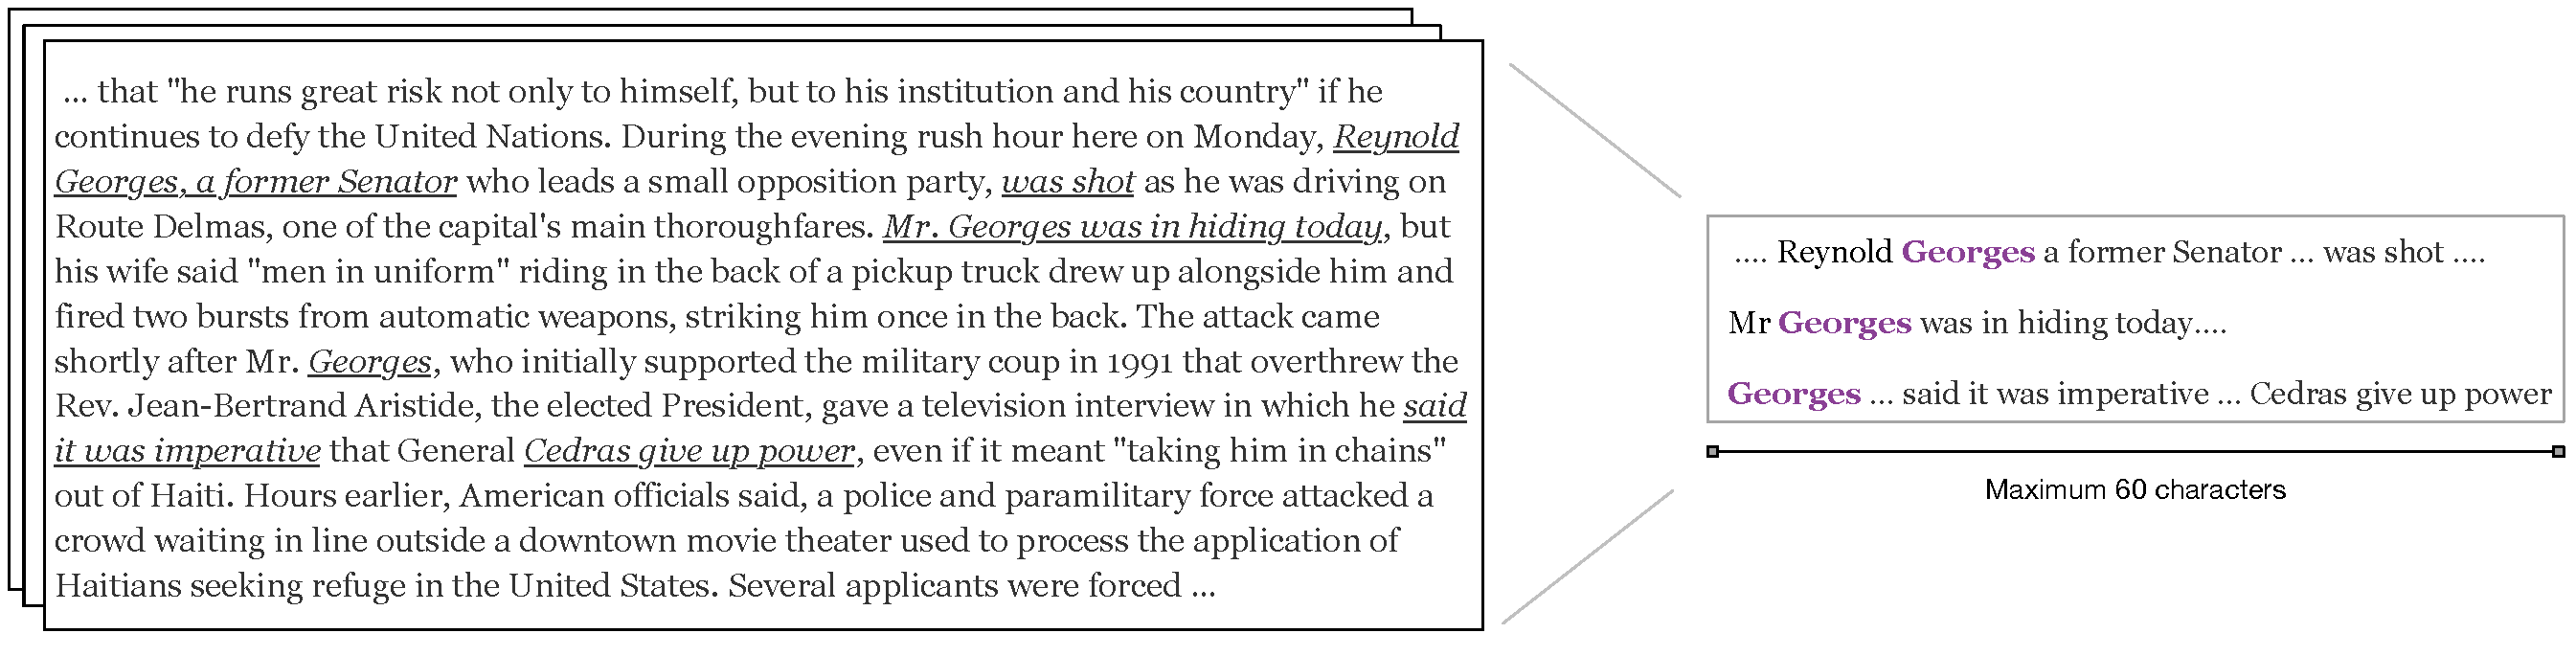
\includegraphics[width=.8\textwidth]{figures/Compression.pdf}
\caption[Text simplification in \ours's Document Feed]{\ours's Document Feed uses text simplification methods from natural language processing in conjunction with color-coded, automatic, in-text highlighting, in order to summarize query mentions \mentions~in context, in a visually consistent format designed for skimming. 
Here one portion of one document (top of stack, left) containing three mentions of the query term $Q$=``Georges'' has been shortened into a summary of ``Georges'' (right). 
To create this summary, \ours~extracts each of the three sentences mentioning ``Georges'' and simplifies each sentence to render a shorter sentence \simplifiedsentence~that is fewer than 60 characters long. 
In this figure, for illustration, spans of tokens from one source document included in the summary are shown with italicized and underlined text. 
In typical use of \ours~there are often hundreds or thousands of documents containing $Q$ (shown as document stack, above left).}\label{f:compressioncartoon}
\end{figure}
